
\begin{flushleft}

\begin{itemize}
	\item Port forwarding is a form of NAT (Network Address Translation). 
	\item With port forwarding, traffic of a server is forwarded either to a different port on the same machine, or to a port on a different machine. 
	\item Port forwarding is used to “hide” a server behind another machine, or to provide access to a service on an alternate port.

	\begin{figure}[h!]
		\centering
		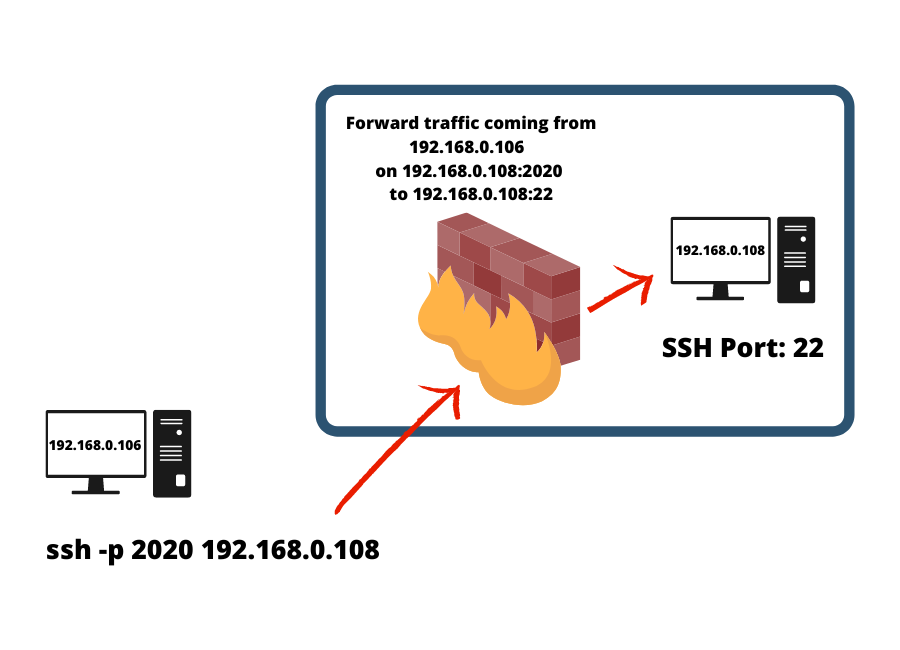
\includegraphics[scale=.3]{content/chapter2/images/port.png}
		\caption{Port forwarding}
		\label{fig:command_prompt12}
	\end{figure}
	
	\bigskip
	\begin{tcolorbox}[breakable,notitle,boxrule=0pt,colback=pink,colframe=pink]
		\color{black}
		\fontdimen2\font=1em
		Syntax: 
		\newline
		firewall-cmd --list-rich-rules
		\fontdimen2\font=4pt
	\end{tcolorbox}
	
	\bigskip
	\bigskip
	\item Add <RICH RULE> to the specified zone, or the default zone if no zone is specified.
	\bigskip
	\begin{tcolorbox}[breakable,notitle,boxrule=0pt,colback=pink,colframe=pink]
		\color{black}
		\fontdimen2\font=1em
		Syntax: 
		\newline
		firewall-cmd --permanent --zone=<ZONE> --add-rich-rule='<RULE>'
		\newline
		firewall-cmd --reload
		\fontdimen2\font=4pt
	\end{tcolorbox}
	
	\bigskip
	\bigskip
	\item Remove <RICH RULE> to the specified zone, or the default zone if no zone is specified.
	\bigskip
	\begin{tcolorbox}[breakable,notitle,boxrule=0pt,colback=pink,colframe=pink]
		\color{black}
		\fontdimen2\font=1em
		Syntax: 
		\newline
		firewall-cmd --permanent --zone=<ZONE> --remove-rich-rule='<RULE>'
		\newline
		firewall-cmd --reload
		\fontdimen2\font=4pt
	\end{tcolorbox}
	
	\newpage
	
	\paragraph{Examples:}
	\bigskip
	\begin{enumerate}
		\item Reject all traffic from a "192.168.0.11/32" IP address in default zone:
		\newline
		Eg:
		\begin{tcolorbox}[breakable,notitle,boxrule=-0pt,colback=black,colframe=black]
			\color{green}
			\fontdimen2\font=1em
			\# firewall-cmd --permanent --add-rich-rule='rule family=ipv4 source address=192.168.0.11/32 reject'
			\newline
			\newline
			\# firewall-cmd --reload
			\fontdimen2\font=4pt
		\end{tcolorbox}
		
		\begin{figure}[h!]
			\centering
			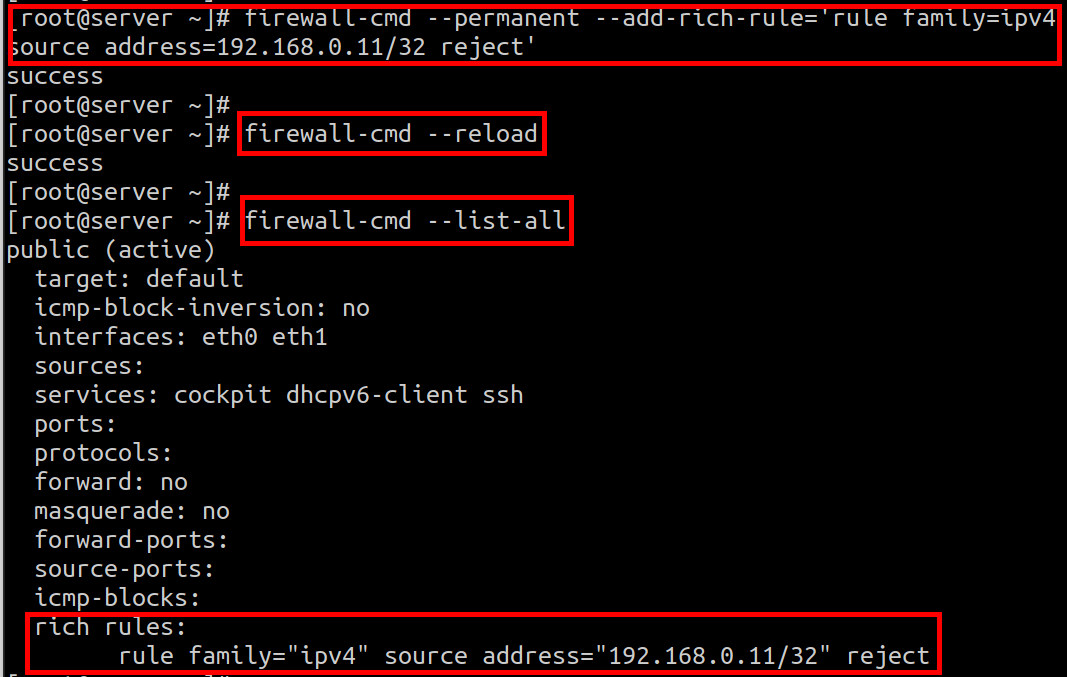
\includegraphics[scale=.3]{content/chapter2/images/zones10.png}
			\caption{Sample output}
			\label{fig:command_prompt7}
		\end{figure}
		
		\newpage
		
		\item Allows port 8080 for a specific IP address "192.168.0.11/32":
		\newline
		Eg:
		\begin{tcolorbox}[breakable,notitle,boxrule=-0pt,colback=black,colframe=black]
			\color{green}
			\fontdimen2\font=1em
			\# firewall-cmd --add-rich-rule='rule family="ipv4" source address="192.168.0.11" port port=8080 protocol=tcp accept'
			\newline
			\newline
			\# firewall-cmd --reload
			\fontdimen2\font=4pt
		\end{tcolorbox}
		
		\begin{figure}[h!]
			\centering
			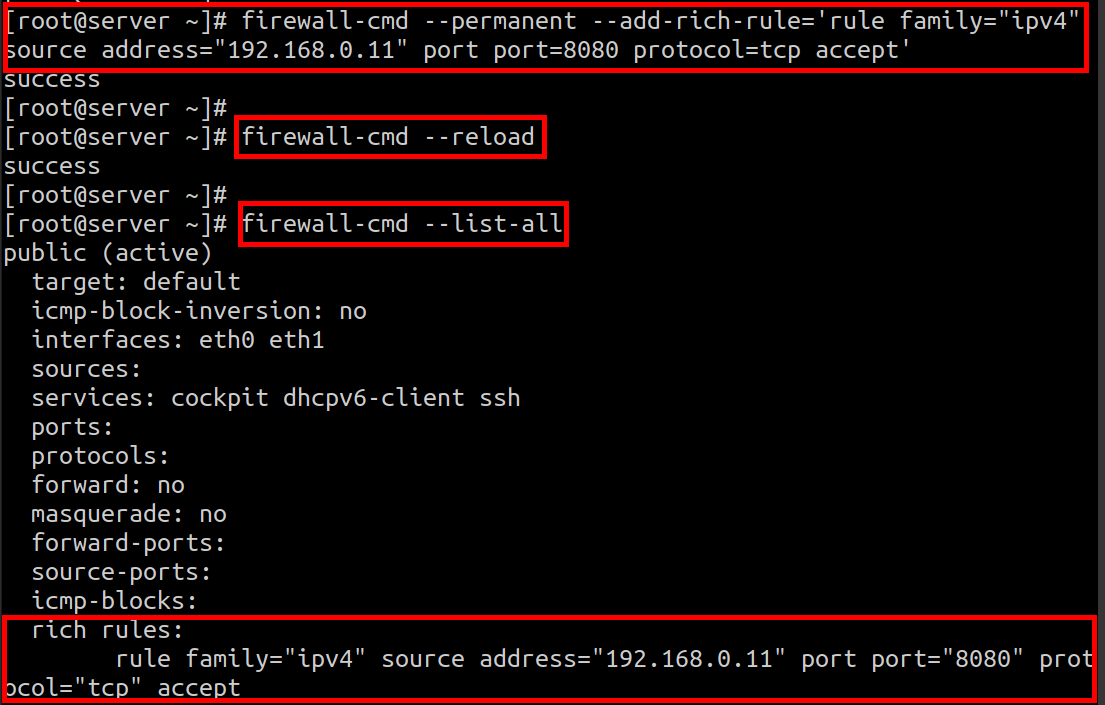
\includegraphics[scale=.3]{content/chapter2/images/zones11.png}
			\caption{Sample output}
			\label{fig:command_prompt9}
		\end{figure}
		
		\newpage
		\item Accept all TCP packets on ports 7900, up to and including port 7905, in the vnc zone for the 192.168.1.0/24 subnet.
		\newline
		Eg:
		\begin{tcolorbox}[breakable,notitle,boxrule=-0pt,colback=black,colframe=black]
			\color{green}
			\fontdimen2\font=1em
			\# firewall-cmd --permanent --zone=vnc --add-rich-rule='rule family=ipv4 source address=192.168.1.0/24 port port=7900-7905 protocol=tcp accept'
			\newline
			\newline
			\# firewall-cmd --reload
			\fontdimen2\font=4pt
		\end{tcolorbox}
		
		\begin{figure}[h!]
			\centering
			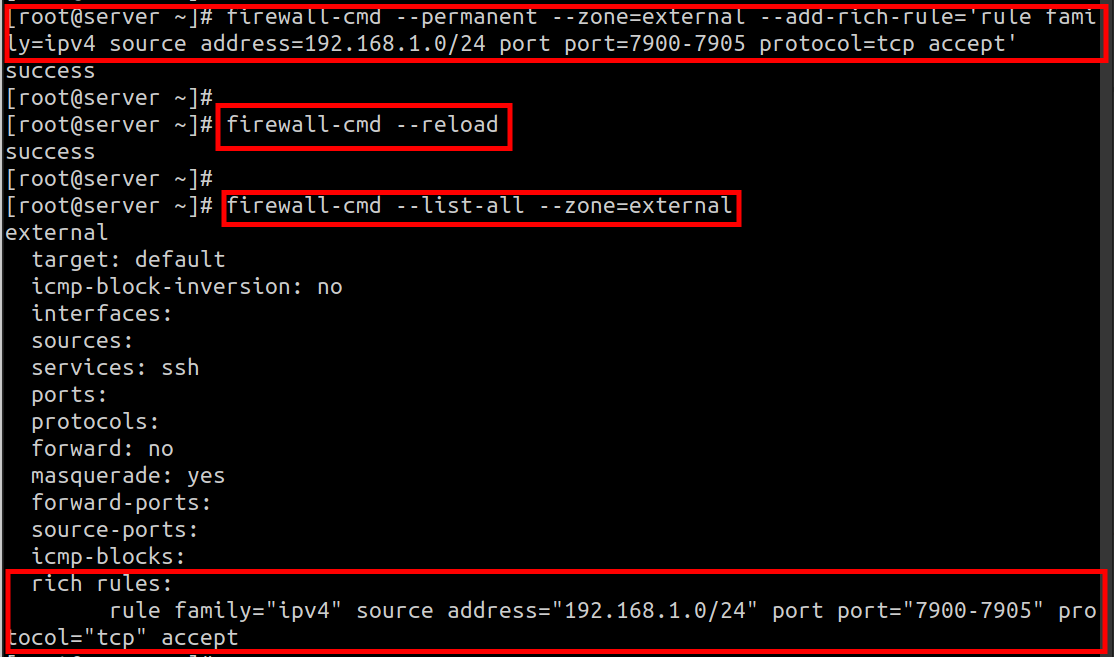
\includegraphics[scale=.3]{content/chapter2/images/zones12.png}
			\caption{Sample output}
			\label{fig:command_prompt10}
		\end{figure}
		
	\end{enumerate}
	
\end{itemize}

	
\end{flushleft}

\newpage





